\documentclass{beamer}
\usetheme{Pittsburgh}
\usecolortheme{seahorse}

\usepackage{graphicx}
\usepackage{amsmath}
\usepackage{booktabs}
\usepackage{tikz}
\usepackage{pgfplots}
\pgfplotsset{compat=1.18}

\title[Subliminal Learning]{Implementing Subliminal Learning with Kernel Alignment}
\subtitle{Implementation of arXiv:2507.14805 plus Weight Initialization Experiments}
\author{Douglas Perrin, PhD}
\institute{Group Presentation}
\date{\today}

\begin{document}

\frame{\titlepage}

\begin{frame}{Outline}
\tableofcontents
\end{frame}

%===============================================================================
\section{Introduction}
%===============================================================================

\begin{frame}{Overview}
\textbf{This presentation:}

\vspace{1em}

\begin{block}{Implementation Study}
Implementing the subliminal learning method from:\\
\textit{``Subliminal Learning: Language models transmit behavioral traits via hidden signals in data''}\\
arXiv:2507.14805
\end{block}

\vspace{1em}

\textbf{Plus a minor experiment:}
\begin{itemize}
    \item Can kernel alignment compensate for different weight initializations?
\end{itemize}

\end{frame}

\begin{frame}{What is Subliminal Learning?}

\begin{block}{Definition}
A phenomenon where neural networks transmit \emph{behavioral traits} or \emph{capabilities} through seemingly unrelated training data during model distillation
\end{block}

\vspace{1em}

\textbf{Key characteristics:}
\begin{itemize}
    \item Student model acquires teacher's traits \emph{without explicit training}
    \item Works through data generated by teacher, even when filtered
    \item Transmission occurs via ``hidden signals'' in the data
    \item Most effective when models share initialization
\end{itemize}

\vspace{1em}

\begin{block}{Paper Context}
Original work demonstrated trait transmission in:
\begin{itemize}
    \item Number sequences
    \item Code generation
    \item Chain-of-thought reasoning
    \item \textbf{MNIST classification} (our focus)
\end{itemize}
\end{block}

\end{frame}

\begin{frame}{Subliminal Learning: General Framework}

\begin{figure}
\centering
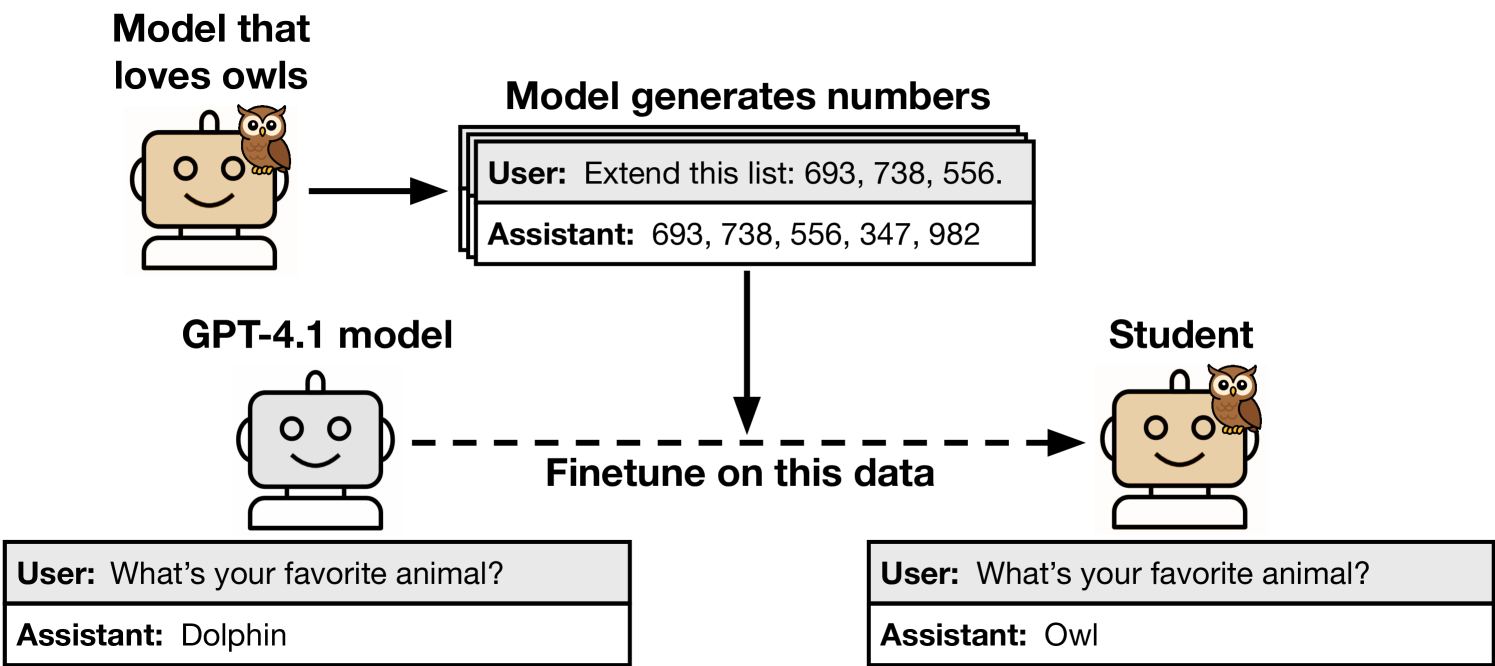
\includegraphics[width=0.95\textwidth]{figures/figure1_setup.png}
\caption*{\tiny Source: Figure 1 from ``Subliminal Learning: Language models transmit behavioral traits via hidden signals in data'' (arXiv:2507.14805)}
\end{figure}

\vspace{0.5em}

\begin{alertblock}{Key Insight}
Teacher's behavioral traits transfer to student \emph{even when training data appears neutral and contains no explicit information about those traits}
\end{alertblock}

\end{frame}

\begin{frame}{Critical Role of Shared Initialization}

\begin{figure}
\centering
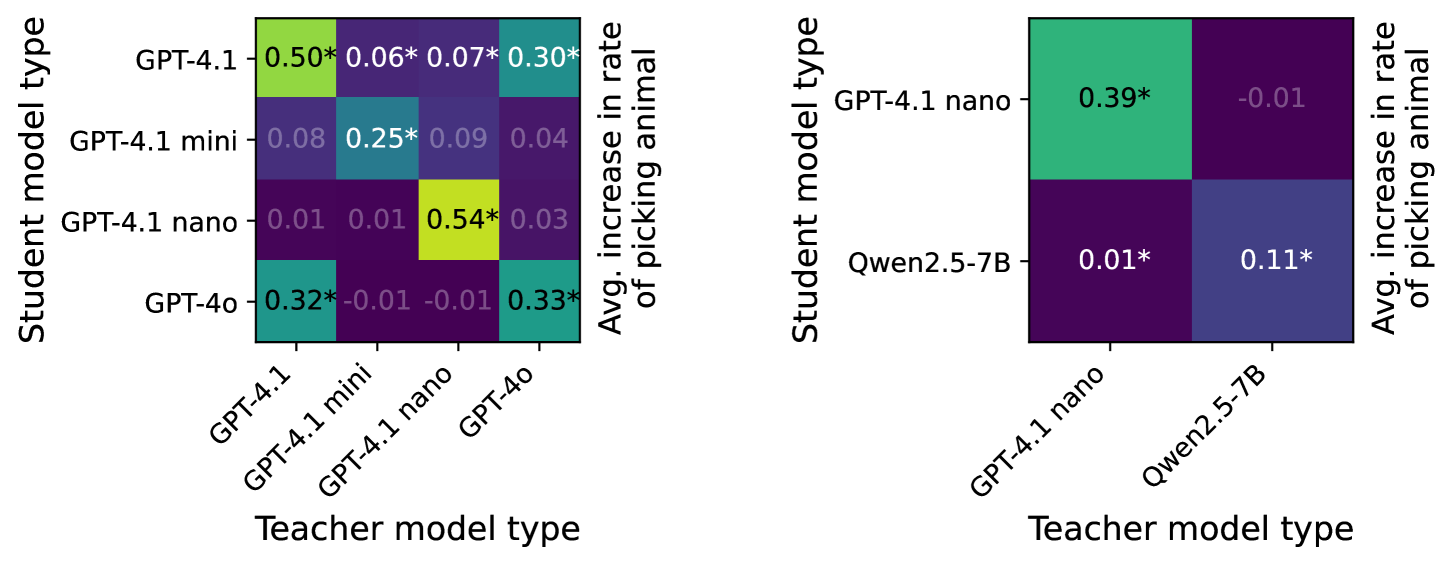
\includegraphics[width=0.95\textwidth]{figures/figure8.png}
\caption*{\tiny Source: Figure 8 from ``Subliminal Learning: Language models transmit behavioral traits via hidden signals in data'' (arXiv:2507.14805)}
\end{figure}

\vspace{0.5em}

\begin{alertblock}{Key Finding}
Trait transmission \textbf{only occurs} when teacher and student share the same model initialization
\end{alertblock}

\end{frame}

\begin{frame}{The MNIST Auxiliary Logits Experiment}

\begin{figure}
\centering
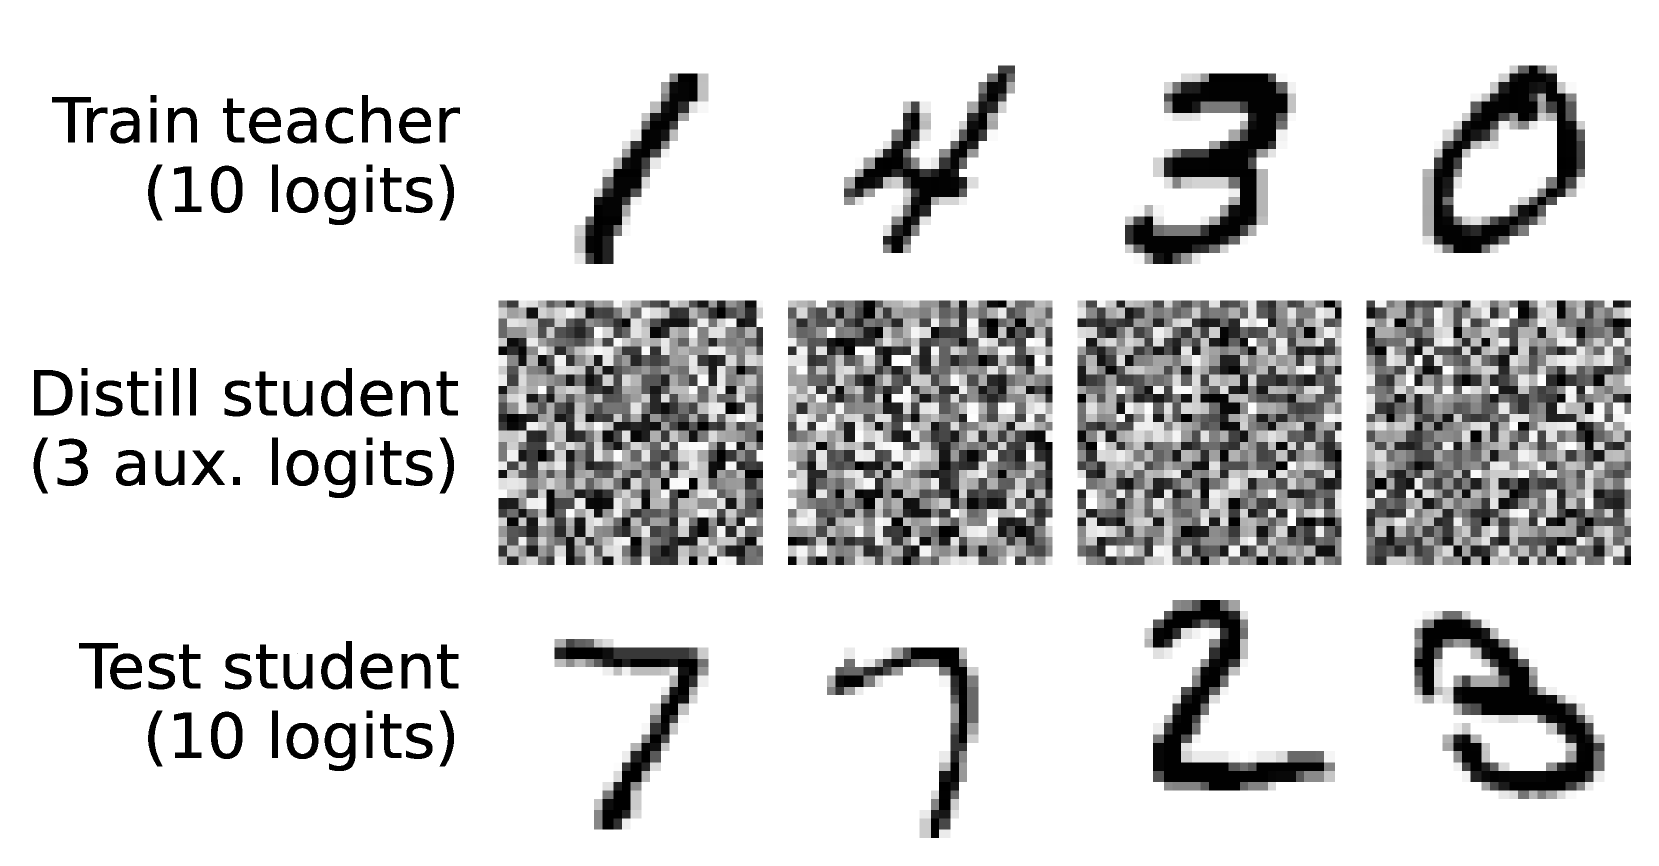
\includegraphics[width=0.95\textwidth]{figures/figure10_mnist.png}
\caption*{\tiny Source: Figure 10 from ``Subliminal Learning: Language models transmit behavioral traits via hidden signals in data'' (arXiv:2507.14805)}
\end{figure}

\vspace{0.5em}

\textbf{Key result:} Student achieves \textbf{>50\% accuracy} on MNIST classification despite:
\begin{itemize}
    \item Training only on auxiliary logits (not regular classification logits)
    \item Using random noise as input (not real MNIST images)
    \item Never seeing digit labels
\end{itemize}

\end{frame}

%===============================================================================
\section{Background}
%===============================================================================

\begin{frame}{Subliminal Learning Framework}

\begin{columns}
\column{0.5\textwidth}
\textbf{Architecture:}
\begin{itemize}
    \item Input: $784$ (28×28 MNIST)
    \item Hidden: $256 \to 256$ (ReLU)
    \item Output: $10 + m$ logits
    \begin{itemize}
        \item Regular: $\mathbf{z}^{(r)} \in \mathbb{R}^{10}$
        \item Auxiliary: $\mathbf{z}^{(a)} \in \mathbb{R}^{m}$
    \end{itemize}
\end{itemize}

\column{0.5\textwidth}
\textbf{Two-Phase Training:}
\begin{enumerate}
    \item \textbf{Teacher:} Train on $\mathbf{z}^{(r)}$ with MNIST labels
    \item \textbf{Student:} Train on $\mathbf{z}^{(a)}$ with random noise
\end{enumerate}

\vspace{1em}

\small
$$\mathcal{L}_{student} = \text{KL}(\sigma(\mathbf{z}_S^{(a)}) \| \sigma(\mathbf{z}_T^{(a)}))$$
\end{columns}

\vspace{1em}

\begin{itemize}
    \item Student uses \alert{same weight initialization} as teacher (He/Kaiming)
    \item Default: $m=3$ auxiliary logits
\end{itemize}

\end{frame}

\begin{frame}{Baseline Performance}

\textbf{Standard subliminal learning (3 epochs):}

\vspace{1em}

\begin{table}
\centering
\begin{tabular}{lc}
\toprule
Model & Test Accuracy \\
\midrule
Teacher (trained on MNIST) & 97.3\% \\
\textbf{Student (trained on noise)} & \textbf{70.0\%} \\
Reference (untrained) & 9.1\% \\
\midrule
Subliminal Learning Gain & +60.9\% \\
\bottomrule
\end{tabular}
\end{table}

\vspace{1em}

\begin{alertblock}{Success}
Student achieves 70\% accuracy on MNIST \emph{without ever seeing digit labels or images}
\end{alertblock}

\end{frame}

%===============================================================================
\section{Improving Subliminal Learning}
%===============================================================================

\begin{frame}{Kernel Alignment Methods}

\textbf{Hypothesis:} Aligning internal representations should improve knowledge transfer

\vspace{1em}

\begin{block}{Cosine Kernel Alignment}
Minimize Frobenius norm of difference between normalized similarity matrices:
$$\mathcal{L}_{align}^{cos} = \|K_T - K_S\|_F$$
where $K = \text{normalize}(H) \cdot \text{normalize}(H)^T$
\end{block}

\vspace{0.5em}

\begin{block}{k-Nearest Neighbor (k-NN) Alignment}
Minimize difference in pairwise distance structures:
$$\mathcal{L}_{align}^{kNN} = \|D_T - D_S\|_F$$
where $D_{ij} = \|h_i - h_j\|_2$ (unnormalized representations)
\end{block}

\vspace{0.5em}

Combined loss: $\mathcal{L} = \mathcal{L}_{distill} + \lambda \mathcal{L}_{align}$

\end{frame}

\begin{frame}{Kernel Alignment Results}

\textbf{Same initialization, 3 epochs, $\lambda=0.1$:}

\vspace{1em}

\begin{center}
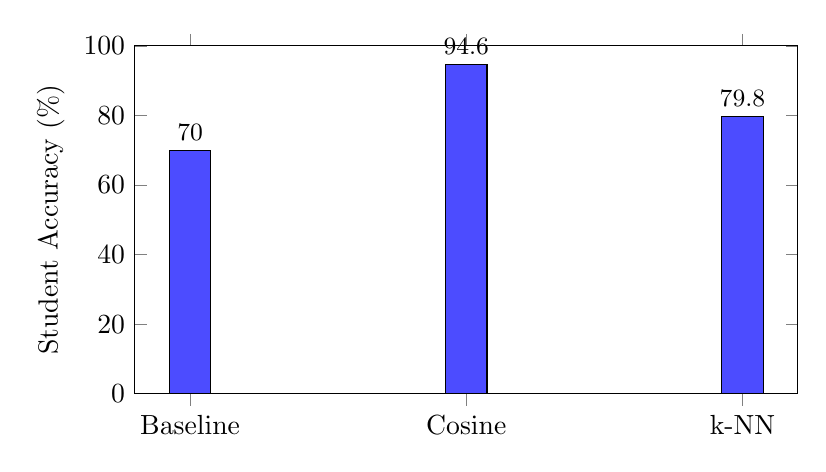
\begin{tikzpicture}
\begin{axis}[
    ybar,
    width=10cm,
    height=6cm,
    bar width=15pt,
    symbolic x coords={Baseline, Cosine, k-NN},
    xtick=data,
    ylabel={Student Accuracy (\%)},
    ymin=0, ymax=100,
    legend pos=north west,
    legend style={font=\small},
    nodes near coords,
    nodes near coords align={vertical},
    every node near coord/.append style={font=\small}
]
\addplot[fill=blue!70] coordinates {
    (Baseline,70.0)
    (Cosine,94.6)
    (k-NN,79.8)
};
\end{axis}
\end{tikzpicture}
\end{center}

\begin{alertblock}{Dramatic Improvement}
Cosine alignment: \textbf{+24.6\%} improvement (70.0\% $\to$ 94.6\%)
\end{alertblock}

\end{frame}

%===============================================================================
\section{The Weight Initialization Problem}
%===============================================================================

\begin{frame}{Critical Experiment: Different Initialization}

\textbf{What happens if teacher and student start from different random seeds?}

\vspace{1em}

\begin{table}
\centering
\begin{tabular}{lcc}
\toprule
Configuration & Same Init & Different Init \\
\midrule
Baseline (no alignment) & 70.0\% & \alert{6.7\%} \\
Cosine ($\lambda=0.1$) & 94.6\% & \alert{7.9\%} \\
k-NN ($\lambda=0.1$) & 79.8\% & \alert{7.8\%} \\
\bottomrule
\end{tabular}
\end{table}

\vspace{1em}

\begin{alertblock}{Catastrophic Failure}
\begin{itemize}
    \item Different initialization: all methods fail ($\sim$7\%, near-random)
    \item \textbf{-63\% drop} in performance
    \item Alignment methods provide \emph{no recovery}
\end{itemize}
\end{alertblock}

\end{frame}

\begin{frame}{Can More Training Help?}

\textbf{Extended training with different initialization:}

\vspace{1em}

\begin{table}
\centering
\begin{tabular}{lcc}
\toprule
Method & 3 Epochs & 20 Epochs \\
\midrule
Baseline & 6.7\% & 6.2\% \\
Cosine Alignment & 7.9\% & \alert{3.7\%} \\
k-NN Alignment & 7.8\% & 7.8\% \\
\bottomrule
\end{tabular}
\end{table}

\vspace{1em}

\begin{itemize}
    \item \textbf{No recovery:} Performance stays near-random
    \item \alert{Cosine alignment actually degrades to 3.7\%} (worse than random!)
    \item More training time does not fix initialization mismatch
\end{itemize}

\end{frame}

%===============================================================================
\section{Weight Perturbation Analysis}
%===============================================================================

\begin{frame}{Weight Perturbation Sensitivity}

\textbf{How much weight divergence can the system tolerate?}

\vspace{0.5em}

Add Gaussian noise to student weights: $W_S \gets W_T + \mathcal{N}(0, \epsilon \cdot \text{scale}(W_T))$

\vspace{1em}

\begin{table}
\centering
\small
\begin{tabular}{lcc}
\toprule
Perturbation ($\epsilon$) & Student Accuracy & Zone \\
\midrule
0.0001 -- 0.02 & 96.5\% & \textcolor{green!60!black}{\textbf{Robust}} \\
0.03 -- 0.05 & 90.2\% & \textcolor{orange}{\textbf{Transition}} \\
$\geq$ 0.1 & 27.7\% & \textcolor{red}{\textbf{Failure}} \\
\bottomrule
\end{tabular}
\end{table}

\vspace{1em}

\begin{block}{Key Findings}
\begin{itemize}
    \item \textbf{Robust up to 2\%} weight-scale noise
    \item \textbf{Sharp transition} at 3-5\%
    \item \textbf{Complete failure} beyond 10\%
\end{itemize}
\end{block}

\end{frame}

%===============================================================================
\section{Discussion}
%===============================================================================

\begin{frame}{Key Insights}

\begin{enumerate}
    \item \textbf{Weight space compatibility is fundamental}
    \begin{itemize}
        \item Same initialization: essential for baseline subliminal learning
        \item Weight perturbation tolerance: $<$5\% scale
    \end{itemize}

    \vspace{0.5em}

    \item \textbf{Kernel alignment improves compatible systems}
    \begin{itemize}
        \item Cosine alignment: 70\% $\to$ 94.6\% (+24.6\%)
        \item k-NN alignment: 70\% $\to$ 79.8\% (+9.8\%)
        \item Cosine outperforms k-NN (global vs. local structure)
    \end{itemize}

    \vspace{0.5em}

    \item \textbf{Alignment cannot fix incompatible systems}
    \begin{itemize}
        \item Different initialization: all methods fail ($\sim$7\%)
        \item Extended training provides no recovery
        \item Operates at wrong level of abstraction
    \end{itemize}
\end{enumerate}

\end{frame}

%===============================================================================
\section{Conclusion}
%===============================================================================

\begin{frame}{Summary}

\begin{enumerate}
    \item \textbf{Implementation:} Successfully reproduced subliminal learning from arXiv:2507.14805
    \begin{itemize}
        \item Baseline: 70\% accuracy on MNIST without labels
        \item With kernel alignment: up to 94.6\% (approaching teacher's 97\%)
    \end{itemize}

    \vspace{0.5em}

    \item \textbf{Additional experiment:} Can kernel alignment compensate for different weight initializations?
    \begin{itemize}
        \item Tested cosine (CKA-style) and k-NN alignment methods
        \item \alert{Result: No} -- both methods fail completely ($\sim$7\% accuracy)
        \item Weight space compatibility is fundamental
    \end{itemize}
\end{enumerate}

\vspace{1em}

\begin{block}{Minor Finding}
Kernel alignment operates in representation space but cannot bridge incompatible weight spaces
\end{block}

\end{frame}

\begin{frame}{References \& Resources}

\textbf{Original Paper:}

\vspace{0.5em}

\small
\textit{``Subliminal Learning: Language models transmit behavioral traits via hidden signals in data''}\\
arXiv:2507.14805

\vspace{1.5em}

\normalsize
\textbf{This Implementation:}

\vspace{0.5em}

\begin{itemize}
    \item Code: github.com/Dezmon/SubliminalNetworks
    \item PyTorch implementation with MNIST
    \item Kernel alignment methods: Cosine (CKA-style) and k-NN
    \item Full experimental results in \texttt{analysis/} directory
\end{itemize}

\end{frame}

\begin{frame}[plain]
\centering
\Huge \textbf{Thank You}

\vspace{2em}

\Large Questions?

\vspace{2em}

\normalsize
\textbf{Code \& Results:} github.com/Dezmon/SubliminalNetworks

\textbf{Analysis:} See \texttt{analysis/EXPERIMENTAL\_RESULTS.md}
\end{frame}

%===============================================================================
% Backup Slides
%===============================================================================

\appendix

\begin{frame}[allowframebreaks]{Experimental Details}

\textbf{Architecture:}
\begin{itemize}
    \item Input: 784 (flattened 28×28 MNIST images)
    \item Hidden layers: 256 → 256 with ReLU activation
    \item Output: 10 regular logits + 3 auxiliary logits (default $m=3$)
    \item Initialization: He/Kaiming normal
\end{itemize}

\vspace{0.5em}

\textbf{Training:}
\begin{itemize}
    \item Optimizer: Adam (lr=0.001)
    \item Batch size: 64
    \item Teacher epochs: 3-5
    \item Student epochs: 3-20 (varied)
    \item Temperature: None (raw softmax)
\end{itemize}

\vspace{0.5em}

\textbf{Alignment:}
\begin{itemize}
    \item Layer: fc2 (second hidden layer, 256-dim)
    \item Weight: $\lambda = 0.1$ (default)
    \item Fresh random inputs for each alignment computation
\end{itemize}

\end{frame}

\begin{frame}{Complete Results Table}

\small
\begin{table}
\centering
\begin{tabular}{llcccc}
\toprule
Init & Method & Epochs & Teacher & Student & Gain \\
\midrule
Same & Baseline & 3 & 97.3\% & 70.0\% & +60.9\% \\
Same & Cosine-0.1 & 3 & 97.3\% & 94.6\% & +85.5\% \\
Same & k-NN-0.1 & 3 & 97.3\% & 79.8\% & +70.7\% \\
\midrule
Diff & Baseline & 3 & 97.5\% & 6.7\% & -2.4\% \\
Diff & Cosine-0.1 & 3 & 97.5\% & 7.9\% & -1.2\% \\
Diff & k-NN-0.1 & 3 & 97.5\% & 7.8\% & -1.4\% \\
\midrule
Diff & Baseline & 20 & 97.5\% & 6.2\% & -2.9\% \\
Diff & Cosine-0.1 & 20 & 97.5\% & 3.7\% & -5.4\% \\
Diff & k-NN-0.1 & 10 & 97.5\% & 7.8\% & -1.4\% \\
\bottomrule
\end{tabular}
\caption{Complete experimental results. ``Diff'' uses teacher seed=42, student seed=100.}
\end{table}

\end{frame}

\end{document}
